\section{Methodology}\label{sec:meto}
% Conceptual explanation of implementation, configuration, and setup. (May use code snippets and
% screenshots to explain concepts, but not full code listings.)
After deciding on our project topic we fixed our software requirements in more concrete form. We identified that it would be most beneficial to divide our future code into frontend and backend with the main interface being between graphical user interface (GUI) and text data structure. The \verb|textStructure.h| header is the main interface connecting the GUI in \verb|main.c| and the actual text data structure implementation in \verb|textStructure.c| \cite{GithubRepo}. The other files are mostly built around these two central pieces of code. A more visual layout can be seen in figure \ref{fig:codeStruct}.
\begin{figure}[H]
\noindent\begin{tikzpicture}[ 
    % Define node styles
    scale = 1,
    node distance = 0.5cm,
    minimum height = 1cm,
    imp/.style={rectangle, rounded corners, fill=teal!65, draw, align=center},
    file/.style={rectangle, rounded corners, fill=teal!25, draw, align=center},
    adj/.style={rectangle, rounded corners, fill=gray!10, draw, align=center},
    division1/.style={rectangle, fill=teal!5, draw=teal!20, line width=1pt, inner sep=5mm},
    division2/.style={rectangle, fill=teal!5, draw=teal!20, line width=1pt, inner sep=5mm},
    division3/.style={rectangle, fill=gray!5, draw=gray!50, line width=1pt, inner sep=5mm},
]

% Main nodes
\node[file] (guiUt) {guiUtilities};
\node[file, right= 1.5of guiUt] (fileM) {fileManager};
\node[file, right= of fileM] (undo) {undoRedoUtilities};
\node[file, right= of undo] (stats) {statistics};

\node[imp, above= of guiUt] (main) {main};
\node[imp, above= of undo] (txtStruct) {textStructure};

\node[adj, right = 1.5of stats] (profiler){profiler};
\node[adj, above= of profiler] (debug) {debugUtil};

% Background division boxes using fit library
\begin{scope}[on background layer]
    \node[division1, fit=(main)(guiUt)] (division1) {};
    \node[above= 0.1of division1] {\bfseries Frontend};
    \node[division2, fit=(txtStruct)(fileM)(undo)(stats)] (division2) {};
    \node[above= 0.1of division2] {\bfseries Backend};
    
    \node[division3, fit=(profiler)(debug)] (division3) {};
    \node[above= 0.1of division3] {\bfseries debugging \& analysis};
\end{scope}

% Arrows for main flow
\draw[latex-latex,  line width=2pt] (main) -- (txtStruct);

\draw[latex-latex,  line width=0.5pt] (main) -- (guiUt);
\draw[latex-latex,  line width=0.5pt] (main) -- (fileM);
\draw[latex-latex,  line width=0.5pt] (txtStruct) -- (fileM);
\draw[latex-latex,  line width=0.5pt] (txtStruct) -- (undo);
\draw[latex-latex,  line width=0.5pt] (txtStruct) -- (stats);

\end{tikzpicture}
\caption{Project Code Structure}
\label{fig:codeStruct}
\end{figure}

The piece table stores the piece descriptors in form of a doubly linked list (see figure \ref{fig:sequence}). Each piece is identified by the buffer it is stored in, the offset into that buffer and its size. Editing the text sequence at a specific position, therefore requires the piece descriptor associated with that position by using the \verb|getNodeForPosition| function. Afterwards, all changes can be done locally around the respective piece descriptor. By using empty sentinel nodes at the beginning and end of the piece table, we can simplify edge cases of changing the sequence at these positions.

\noindent
\\The add buffer grows dynamically with the amount of content it stores. Since it is append-only, undo and redo can be easily implemented by storing the first and last piece descriptors associated with a changed span of text (see \verb|undoRedoUtilities.c| \cite{GithubRepo}) and the required pointers if and operation should be undone. Multiple operations can also be bundled together by pointing to the previous operation so that they are all undone at the same time (e.g. replace consisting of a deletion followed by an insertion). \\
When searching for a specific text, the main challenge is to keep track of the line numbers because the GUI should directly jump to the result if one is found. Since the sequence is searched linearly in most use cases, we use a cache that stores the position and line number of the last result. While searching, the amount of line breaks after the position where the search should begin is also tracked. By accessing the cached last result, this allows the line number to be determined efficiently. The statistics (word and line count) are initialized when loading the file and then updated dynamically based only on the text that is edited (see \verb|statistics.c| \cite{GithubRepo}). 

\noindent
\\In section 4 it can be seen that the described approach performs fairly well - even for large files and large piece tables.

\begin{figure}[H]
\centering
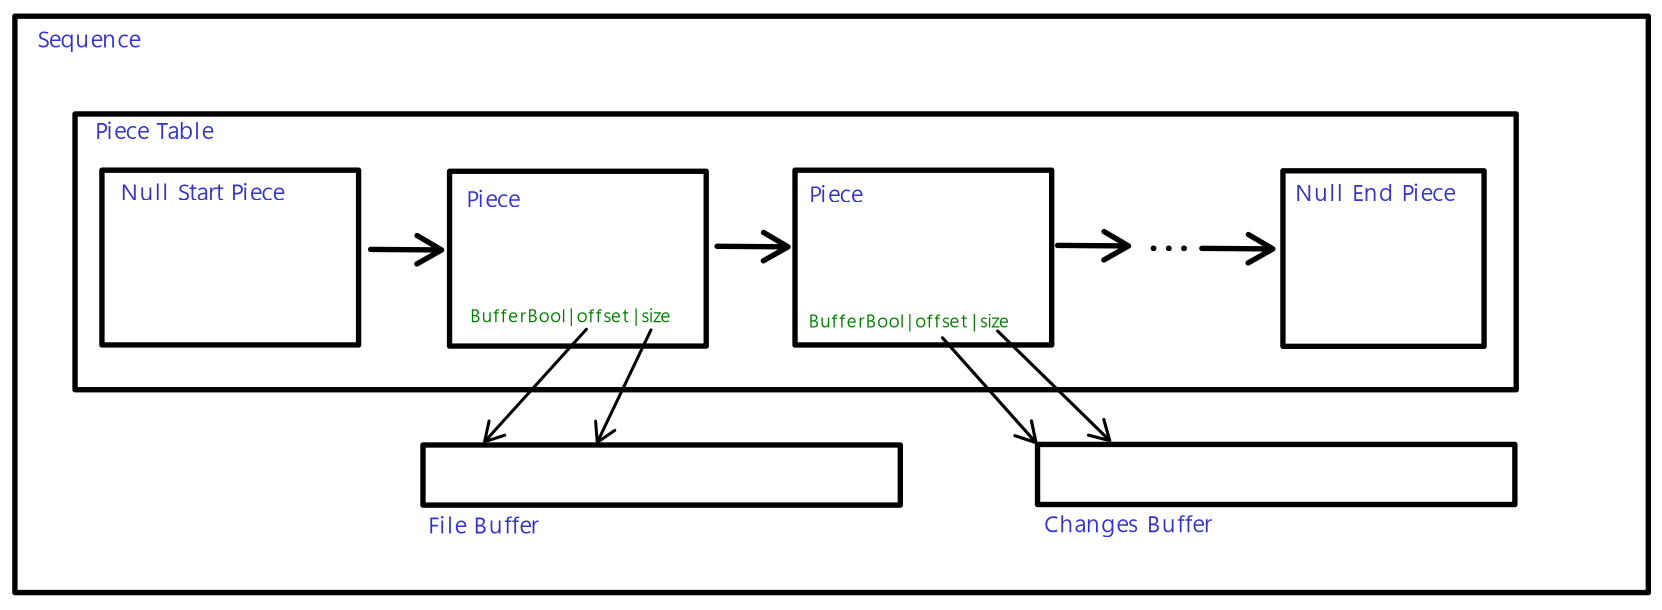
\includegraphics[width=0.8\textwidth]{./images/sequenceIllustration.png}
\caption{High level text data structure (sequence) illustration}
\label{fig:sequence}
\end{figure}

Regarding file management (see \verb|fileManager.c| \cite{GithubRepo}), the way we load files into the editor is optimized even for very large files (we tested up to 5.5 GB text files). That is partly because we directly map the file buffer of the sequence onto a mmap of the opened file. This directly leverages the speed and advantage of the Linux mmap capabilities. Upon save, we also use mmaps to write, but we decided to still take the slight overhead of copying the original file to a temporary location in order to keep the sequence's piece table in its current state and therefore also the whole undo history alive. Otherwise, it would need to be reset each time a save is done, which we found not very user-friendly. 

%GUI
\noindent
\\On the frontend side, \verb|print_items_after| is one of our most important parts and the function that displays text in the terminal. It prints a certain number of lines starting from a chosen atomic position in our text sequence.
This is done by walking through blocks of text data (each block is the span that belongs to a piece descriptor) and handling UTF-8 character boundaries, skipping control characters and detecting line breaks or end-of-block to finish a text line.
It also changes the current line segment to wide-character string for terminal compatibility.
The output is then the processed string that goes to the terminal at the correct screen position.
\\For efficiency, the function only prints lines that are actually visible on the terminal, so lines that are out of view do not get printed. For that we have a variable that has the absolute position of the line at the top of the screen (e.g. top line is actually the 5th line in the entire text).
Also, this is where the line stats get updated and if a line goes across multiple blocks, the counters (\verb|atomicsInLine|, \verb|nbrOfUtf8CharsNoControlCharsInLine|) carry over to the next block.
\\
\\In \verb|guiUtilities| we have functionality for line statistics like getting the current line number at the top of the screen or the amount of characters in a specified line. These methods are used for scrolling, jumping to a specific line when using the search function or managing the line stats.
Characters are the converter from UTF-8 to wide characters and a way to translate cursor position to a position in our data structure.
\\
\\Our cursor refreshes independently of the text. This means that when our cursor moves a position it doesn't cause the text to be refreshed, since that would be a big performance hit.